\documentclass{article}
\usepackage[final]{neurips_2026}

\usepackage[utf8]{inputenc}
\usepackage[T1]{fontenc}
\usepackage{hyperref}
\usepackage{url}
\usepackage{booktabs}
\usepackage{amsfonts}
\usepackage{nicefrac}
\usepackage{microtype}
\usepackage{xcolor}
\usepackage{graphicx}
\usepackage{amsmath}

\title{Structured AutoResearch for Interpretable Marketing Mix Modeling}

\author{%
  Ashley Qiu \\
  STAT 390 \\
  Northwestern University \\
  \texttt{ashley.qiu@u.northwestern.edu}
}

\begin{document}

\maketitle

\begin{abstract}
This report studies whether a structured AutoResearch workflow can improve the predictive accuracy of an interpretable marketing mix model without giving up business readability. The task is to predict geo-level revenue from weekly marketing spend and control variables in Google Meridian sample data using a fixed validation split and validation RMSE as the primary metric. Starting from a simple linear regression baseline with RMSE 73397.18, the controlled search process produced a bounded ridge regression champion with RMSE 69367.07, an absolute improvement of 4030.12 and a relative improvement of 5.49\%. The final result suggests that agent-assisted model search was useful in this setting when the data pipeline, evaluation loop, and allowable model changes were tightly constrained.
\end{abstract}

\section{Introduction}

Marketing teams routinely allocate budget across multiple channels, but the relationship between spend and business outcomes is often difficult to explain from raw data alone. This project frames that problem as an interpretable revenue prediction task: estimate geo-level revenue from weekly marketing spend and control variables while preserving a model structure that remains readable to a marketer. The repository was designed with two linked goals. At the repository level, it provides a reusable workflow that another marketer could adapt to similar data. At the agent level, it asks whether an AutoResearch loop can lower validation RMSE while staying inside a constrained, linear, business-readable model class.

The resulting project is not a search over arbitrary machine learning methods. Instead, it is a controlled sequence of small model revisions made to a single editable file, \texttt{model.py}, while the rest of the experimental environment remains fixed. This structure makes the project suitable for a short NeurIPS-style case study because it combines a clear baseline, a reproducible loop, logged intermediate experiments, and a final model whose feature set can still be interpreted directly. The main contribution of the project is therefore procedural as well as empirical: it shows how a constrained agent-assisted workflow can improve a simple marketing model without drifting into a black-box predictor.

\section{Dataset and Evaluation}

\subsection{Dataset and task}

The report uses \texttt{data/geo\_all\_channels.csv}, a geo-week panel from Google's Meridian sample data included in the repository. The file contains 6240 rows and 20 columns, covering 40 geographies over 156 weekly periods from January 25, 2021 through January 15, 2024. Each row corresponds to one geography in one week and includes channel impressions, channel spend, a promotion indicator, competitor and sentiment controls, conversions, revenue per conversion, and population. The modeling target is revenue, constructed in \texttt{prepare.py} as conversions multiplied by revenue per conversion.

\begin{table}[t]
\centering
\caption{Dataset and task summary.}
\label{tab:data-summary}
\begin{tabular}{ll}
\toprule
Dataset file & \texttt{data/geo\_all\_channels.csv} \\
Rows $\times$ columns & 6240 $\times$ 20 \\
Time unit & Weekly \\
Geographies & 40 \\
Time range & 2021-01-25 to 2024-01-15 \\
Prediction target & Revenue = conversions $\times$ revenue per conversion \\
Primary metric & Validation RMSE \\
Secondary metric & Validation $R^2$ \\
\bottomrule
\end{tabular}
\end{table}

\subsection{Baseline model and fixed evaluation}

The canonical baseline is \texttt{baseline\_model.py}, a simple \texttt{LinearRegression} pipeline with geo one-hot effects, five current-week spend variables, five one-week lagged spend variables, and four controls: \texttt{competitor\_sales\_control}, \texttt{sentiment\_score\_control}, \texttt{Promo}, \texttt{week\_sin}, and \texttt{week\_cos}. This baseline was chosen as a transparent starting point rather than as a strong final model.

Evaluation was frozen in \texttt{prepare.py}. After sorting within geography, the code creates lagged spend features, fixed-decay adstock features, and simple seasonal controls. The first row of each geography is dropped because lagged features are undefined there. A time-based holdout then reserves the final 20\% of periods for validation, giving 4960 training rows and 1240 validation rows. Validation RMSE is the optimization target throughout the project, with $R^2$ recorded as a secondary descriptive metric.

\section{AutoResearch Loop Design}

The AutoResearch loop was intentionally narrow. According to \texttt{README.md} and \texttt{program.md}, \texttt{prepare.py}, \texttt{run.py}, and the dataset were treated as frozen, while \texttt{model.py} was the only editable modeling file. Each session began by logging a session baseline, after which the agent proposed one change at a time, ran the updated model, and compared the new validation RMSE to the best earlier non-discard result in the active session. This design kept all accepted and rejected ideas on a common validation split and produced a complete experiment trail in numbered \texttt{results\_<n>.tsv} files.

\subsection{Allowed search space}

The search space was constrained to interpretable linear modeling choices rather than unrestricted machine learning. The allowed transformations included feature selection over the frozen marketing feature library exposed by \texttt{prepare.py}, channel-specific lag or adstock choices, constrained regularized linear models, and a small number of promotion-by-channel interactions. In practical terms, the project searched over linear pipelines whose coefficients could still be read directly, instead of allowing more flexible but opaque estimators. One especially important design choice was the use of nonnegative bounds on media-related coefficients in later models so that the fit could not imply that spending more on a channel directly reduced revenue.

\subsection{Failure analysis and reflection}

The repository also documents where the loop needed human adjustment. The original rules were narrower through Session 6, then expanded in Session 7 to allow broader feature subset search, regularization, and limited promotion-media interactions. After Session 7, the rules were tightened again because custom post-preprocessor interaction features made coefficient names harder to trace cleanly from the fitted model to the final interpretation. This sequence is a useful lesson from the project itself: AutoResearch was most effective when the loop was tightly structured, but it still benefited from human decisions about what kinds of model changes were admissible and interpretable.

\section{Experimental Results}

\subsection{Baseline versus final model}

Table~\ref{tab:baseline-final} summarizes the main quantitative result. The baseline RMSE of 73397.18 came from the canonical \texttt{LinearRegression} pipeline in \texttt{baseline\_model.py}. The final champion in \texttt{model.py} is a bounded ridge regression pipeline with geo one-hot effects, selected adstock media terms, one promotion interaction, and simple controls. Its final validation RMSE was 69367.07. Relative to baseline, that is an improvement of 4030.12 RMSE points, or 5.49\%.

\begin{table}[t]
\centering
\caption{Baseline and final model comparison.}
\label{tab:baseline-final}
\begin{tabular}{lrr}
\toprule
Model & Validation RMSE & Validation $R^2$ \\
\midrule
Baseline \texttt{LinearRegression} & 73397.18 & 0.6569 \\
Final bounded ridge champion & 69367.07 & 0.6935 \\
\midrule
Absolute RMSE improvement & \multicolumn{2}{r}{4030.12} \\
Percent RMSE improvement & \multicolumn{2}{r}{5.49\%} \\
\bottomrule
\end{tabular}
\end{table}

\subsection{Milestone experiments}

The improvement did not come from one isolated jump. It emerged through several structural changes that were kept across sessions. First, replacing the unconstrained baseline with a bounded linear model that enforced nonnegative media effects reduced RMSE to 69820.12. Second, replacing simple lag terms with adstock carryover features further reduced RMSE to 69643.24. Third, allowing channel-specific carryover choices brought the best pre-interaction model down to 69577.32. Fourth, adding a single bounded \texttt{Promo $\times$ Channel4} interaction improved RMSE to 69452.27. Finally, mild bounded ridge regularization on the no-sentiment interaction champion produced the best observed result of 69367.07.

\begin{table}[t]
\centering
\caption{Selected milestone experiments from the cumulative log.}
\label{tab:milestones}
\begin{tabular}{p{0.56\linewidth}r}
\toprule
Milestone experiment & RMSE \\
\midrule
Baseline linear model & 73397.18 \\
Bounded linear model with nonnegative media effects & 69820.12 \\
Adstock carryover model with decay 0.7 & 69643.24 \\
Channel-specific shorter carryover for Channels 3 and 4 & 69577.32 \\
Bounded \texttt{Promo $\times$ Channel4} interaction & 69452.27 \\
Final bounded ridge champion & 69367.07 \\
\bottomrule
\end{tabular}
\end{table}

\begin{figure}[t]
\centering
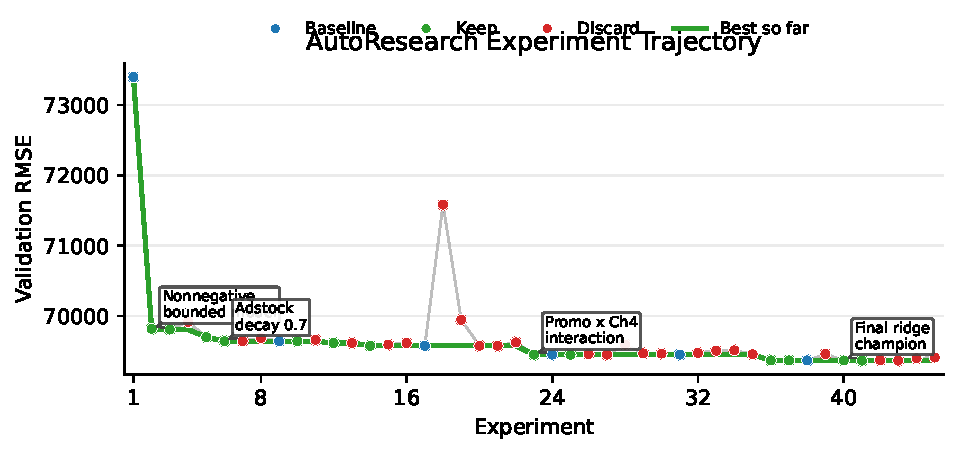
\includegraphics[width=\linewidth]{figures/cumulative_rmse.pdf}
\caption{Cumulative experiment trajectory built from \texttt{results\_cumulative.tsv}. Colored points denote session baselines, kept changes, and discarded changes, while the green line tracks the best-so-far RMSE.}
\label{fig:cumulative-rmse}
\end{figure}

\subsection{Final model interpretation and stability}

The final model remained compact enough to interpret directly. Its retained media features were \texttt{Channel0\_spend\_adstock\_07}, \texttt{Channel1\_spend\_adstock\_07}, \texttt{Channel2\_spend\_adstock\_07}, and \texttt{Channel4\_spend\_adstock\_03}, along with the interaction \texttt{Channel4\_spend\_adstock\_03 $\times$ Promo}. It also included \texttt{competitor\_sales\_control}, \texttt{Promo}, \texttt{week\_sin}, and \texttt{week\_cos}. This means the final model favored a smaller subset of carryover-adjusted marketing terms rather than using every raw spend channel, every lag term, or every transformed feature available in the library.

That compactness supports a readable business interpretation. The strongest positive media signal came from the Channel 2 adstock term, the Channel 4 interaction suggested that Channel 4 spend became more valuable during promotion weeks, and the exclusion of raw spend variables implied that the data was better explained by effects that persisted over time rather than by same-week spend alone. The later sessions also suggest a degree of stability. After the major gains from bounded constraints, adstock, and the promotion interaction, the last improvements were incremental refinements rather than major reversals of model structure. This pattern is consistent with the repository's own memo that the search was approaching the lower end of what this frozen, interpretable linear space could support.

\section{Conclusion}

This project started from a simple linear marketing baseline and used a structured AutoResearch loop to improve validation RMSE while preserving interpretability. The final result reduced RMSE from 73397.18 to 69367.07, an absolute improvement of 4030.12 and a relative improvement of 5.49\%. Just as importantly, the final model remained reproducible and readable: it is still a linear pipeline whose main media effects, carryover assumptions, and one promotion interaction can be inspected directly.

The broader lesson is that agent-assisted research worked best here when the project was tightly structured. Freezing the data preparation, split, and evaluation loop made experiment results comparable across sessions, and limiting the editable search to \texttt{model.py} prevented drift into uncontrolled changes. At the same time, the project also shows the limits of metric-driven search. Human oversight was still needed to revise the search rules, constrain the model family, and keep later interaction features traceable enough for final interpretation. For marketing mix modeling in particular, that balance between optimization and readability appears to be the central design challenge.

% References and checklist are kept as separate report assets and are not
% included in the default compiled PDF so the submission stays within the
% intended 4-page main report.

\end{document}
